\documentclass[a4paper,11pt]{article}
\usepackage[utf8]{inputenc}
\usepackage[russian]{babel}
\usepackage[T1]{fontenc}
\usepackage{amssymb,amsmath,clrscode,graphicx,indentfirst}

\author{Иван Веселов}
\title{Курс kiev-clrs -- Лекция 3. ``Разделяй и властвуй''}
\date{2009 г.}

\begin{document}

\maketitle
\tableofcontents
\newpage

\setlength{\parskip}{1ex plus 0.5ex minus 0.2ex}

\section{Рассматриваемые алгоритмы}
\begin{itemize}
\item Бинарный поиск
\item Возведение в степень
\item Числа Фибоначчи
\item Умножение матриц
\item Алгоритм Страссена
\item Размещение деревьев на БИСМ (VLSI)
\end{itemize}

\section{Описание метода}

Нюанс перевода: ``divide and conquer'' -- переводится обычно как ``разделяй и
властвуй'', хотя дословно будет ``разделяй и покоряй''.

\begin{enumerate}
\item разделяй (divide) -- разделение задачи (её конкретного экземпляра) на
  подзадачи, как правило меньшего размера
\item покоряй (conquer) -- рекурсивное решение подзадач
\item властвуй (combine) -- объединение полученных решений подзадач.
\end{enumerate}

В силу специфики этого метода оценка времени выполнения всегда будет
представляться в виде рекуррентности, которая подходит для основного метода, то
есть рекуррентности вида:

$T(n) = aT(n/b) + f(n)$,

где $a$ -- количество подзадач,

$n/b$ -- размер подзадачи

$f(n)$ -- работа, которая тратится на разделение и объединение

\section{Сортировка слиянием}

Рассмотрим пример из предыдущей лекции: сортировку слиянием.
\begin{enumerate}
\item разделение: тривиально, просто выбираем элемент в центре массива и считаем
  что мы разделили массив
\item покорение: рекурсивно сортируем два получившихся подмассива
\item объединение: слияние за линейное время $\Theta(n)$
\end{enumerate}

Получаем рекуррентность $T(n) = 2T(n/2) + \Theta(n)$, её решением согласно
второму случаю основной теоремы будет $\Theta(n log(n))$

\section{Основная теорема (напоминание)}

При использовании основного метода функция $f(n)$ сравнивается с $n^{\log_b a}$
и рассматриваются три случая. Интуитивно понятно, что асимптотическое поведение
решения рекуррентного соотношения определяется большей из двух функций.

\begin{enumerate}
\item Если $f(n) = O(n^{\log_{b}{a - \epsilon}})$ , для некоторой константы
  $\epsilon > 0$, т.е. $f(n)$ растет полиноминально медленней чем
  $n^{\log_b a}$ в $n^\epsilon$ раз.\\
  Тогда $T(n) = \Theta(n^{\log_b a})$

\item Если $f(n) = \Theta(n^{\log_b a}\lg^k n)$, т.е. $f(n)$ и $n^{log_b a}$
  растут с одинаковой скоростью с точностью до множителя $\lg^k n$, для
  константы $k \geqslant 0$.\\ Тогда $T(n) = \Theta(n^{\log_b a} \lg^{k+1} n)$

\item Если $f(n) = \Omega(n^{\log_b{a + \epsilon}})$ , для некоторой константы
  $\epsilon > 0$, т.е. $f(n)$ растет полиноминально быстрей чем $n^{\log_b a}$
  в $n^\epsilon$ раз \\ \emph{и} $f(n)$ удовлетворяет неравнеству $a f(n/b)
  \leqslant c f(n)$ для некоторого $c < 1$ \\ Тогда $T(n) = \Theta(f(n))$
\end{enumerate}

В сортировке слиянием $a = 2, b = 2, f(n) = \Theta(n)$, то есть нам нужно
сравнить $\Theta(n)$ и $n^{\log_2 2} = n^1 = n$. Они апроксиматически равны
(случай 2 теоремы, $k = 0$), таким образом ответом будет $T(n) = \Theta(n \lg
n)$

\section{Бинарный поиск}

Задача: найти элемент в отсортированном массиве.

\begin{enumerate}
\item разделение -- сравнение со средним элементом и последующий выбор
  подмассива
\item покорение -- поиск в одном подмассиве
\item объединение -- тривиальное (ничего не надо делать)
\end{enumerate}

Оценка времени выполнения: $T(n) = T(n/2) + \Theta(1)$ (одно подзадача, в два
раза меньше основной задачи и константное время для объединения), снова второй
случай основной теоремы и решение $T(n) = \Theta(\lg n)$

\section{Возведение в степень}

Задача: найти целую степень числа, то есть найти $a^n, \text{ где } n \in
\mathbb{N}$

Наивный алгоритм: $\Theta(n)$

Алгоритм ``разделяй и властвуй'':

\begin{equation*}
  a(n) = \begin{cases}
  a^{n/2} a^{n/2}, \text{ если n -- чётное} \\
  a^{(n-1)/2} a^{(n-1)/2} a,  \text{ если n -- нечётное}
  \end{cases}
\end{equation*}

Время работы: $T(n) = T(n/2) + \Theta(1) \Rightarrow T(n) = \Theta(\lg n)$

\section{Числа Фибоначчи}

Рекурсивное определение:
\begin{equation*}
  F_n = \begin{cases}
  0, \text{ если } n = 0 \\
  1, \text{ если } n = 1 \\
  F_{n-1} + F_{n-2}, \text{ если } n > 1
  \end{cases}
\end{equation*}

Наивный рекурсивный алгоритм: $\Omega(\phi^n)$, где $\phi$ -- золотое сечение.
Экспоненциальное время работы -- очень плохо.

Итеративный алгоритм: последовательно считать $F_0, F_1, F_2, \ldots$ для
получения нового числа складывать два предыдущих -- на каждое число одно
сложение, значит время выполнение $T(n) = \Theta(n)$

Наивное возведение в степень: мы можем использовать известную формулу: $F_n =
\phi^n / \sqrt{5}$, округлённое в сторону ближайшего целого. Используя оценку из
предыдущего раздела, получим время выполнения $\Theta(\lg n)$. Однако этот метод
не слишком надёжный, т.к. из-за ошибок округления вещественных чисел можем
получить неверный результат.

Теорема:

\begin{equation*}
\begin{bmatrix}
  F_{n+1} & F_n \\
  F_n     & F_{n-1}
\end{bmatrix} =
\begin{bmatrix}
  1 & 1 \\
  1 & 0
\end{bmatrix}^n
\end{equation*}

Алгоритм: рекурсивное возведение в квадрат (то же, что применялось для
возведения в степень). Его оценка как известно $\Theta(\lg n)$
Возведение матрицы 2 на 2 в квадрат асимптотически ничем не отличается от
возведения числа в квадрат, просто вместо одного умножения придётся делать
восемь и ещё четыре сложения, но все равно константное время $\Theta(1)$

Доказательство теоремы (индукция по $n$):

Базис ($n=1$)
\begin{equation*}
\begin{bmatrix}
  F_2 & F_1 \\
  F_1 & F_0
\end{bmatrix} =
\begin{bmatrix}
  1 & 1 \\
  1 & 0
\end{bmatrix}^1
\end{equation*}

Индукция (для $n > 1$):
\begin{equation*}
\begin{bmatrix}
  F_{n+1} & F_n \\
  F_n     & F_{n-1}
\end{bmatrix} =
\begin{bmatrix}
  F_n     & F_{n-1} \\
  F_{n-1} & F_{n-2}
\end{bmatrix}
\begin{bmatrix}
  1 & 1 \\
  1 & 0
\end{bmatrix} =
\begin{bmatrix}
  1 & 1 \\
  1 & 0
\end{bmatrix}^{n-1}
\begin{bmatrix}
  1 & 1 \\
  1 & 0
\end{bmatrix} =
\begin{bmatrix}
  1 & 1 \\
  1 & 0
\end{bmatrix}^n
\end{equation*}

\section{Умножение матриц}
Вход: $A = [a_{ij}], B = [b_{ij}]$

Выход: $C = [c_{ij}] = A \cdot B, i \in 1 \ldots n$

\begin{equation*}
\begin{pmatrix}
c_{11} & c_{12} & \ldots & c_{1n} \\
c_{21} & c_{22} & \ldots & c_{2n} \\
\vdots & \vdots & \ddots & \vdots \\
c_{n1} & c_{n2} & \ldots & c_{nn}
\end{pmatrix}
=
\begin{pmatrix}
a_{11} & a_{12} & \ldots & a_{1n} \\
a_{21} & a_{22} & \ldots & a_{2n} \\
\vdots & \vdots & \ddots & \vdots \\
a_{n1} & a_{n2} & \ldots & a_{nn}
\end{pmatrix}
\cdot
\begin{pmatrix}
b_{11} & b_{12} & \ldots & b_{1n} \\
b_{21} & b_{22} & \ldots & b_{2n} \\
\vdots & \vdots & \ddots & \vdots \\
b_{n1} & b_{n2} & \ldots & b_{nn}
\end{pmatrix}
\end{equation*}

Формула для нахождения элементов матрицы произведения:
\begin{equation*}
c_{ij} = \sum_{k=1}^n a_{ik} b_{kj}
\end{equation*}

Наивный алгоритм на псевдокоде:

\begin{codebox}
\li \For $i \gets 1 $ \To $n$
\li     \Do \For $j \gets 1 $ \To $n$
\li         \Do $c_{ij} \gets 0$
\li             \For $k \gets 1 $ \To $n$
\li             \Do $c_{ij} \gets c_{ij} + a_{ik} b_{kj}$
                \End
            \End
        \End
\end{codebox}

Три вложенных цикла, таким образом сложность вычислений $\Theta(n^3)$

Теперь алгоритм в стиле ``разделяй и властвуй''. Идея:

Представим, что матрица $n \times n$ -- это $2 \times 2$-матрица $(n/2) \times
(n/2)$ подматриц:

\begin{equation*}
\begin{split}
\begin{bmatrix}
  r & s \\
  t & u
\end{bmatrix}
&=
\begin{bmatrix}
  a & b \\
  c & d
\end{bmatrix}
\cdot
\begin{bmatrix}
  e & f \\
  g & h
\end{bmatrix} \\
C &= A \cdot B
\end{split}
\end{equation*}

\begin{equation*}
\text{ 8 \emph{рекурсивных} умножений + 4 сложения матриц } 2 \times 2
\begin{cases}
  r = ae + bg \\
  s = af + bh \\
  t = ce + dg \\
  u = cf + dh
\end{cases}
\end{equation*}

Получим такую рекуррентность: $T(n) = 8T(n/2) + \Theta(n)$

Нужно сравнить $n^{\log_2 8}$ и $\Theta(n)$. Первое полинамильно больше,
получаем первый случай основной теоремы и стало быть решение: $T(n) =
\Theta(n^3)$

Неожиданно! Решение оказалось точно таким же, как и оригинальное :)

\section{Алгоритм Штрассена}
Умножить матрицы $2 \times 2$ с помощью семи перемножений, а не восьми.

$$P_1 = a(f - h)$$
$$P_2 = (a + b)h$$
$$P_3 = (c + d)e$$
$$P_4 = d(g - e)$$
$$P_5 = (a + d)(e + h)$$
$$P_6 = (b - d)(g + h)$$
$$P_7 = (a - c)(e + f)$$

А потом можно посчитать $r, s, t, u$ с помощью таких формул:

$$r = P_5 + P_4 - P_2 + P_6$$
$$s = P_1 + P_2$$
$$t = P_3 + P_4$$
$$u = P_5 + P_1 - P_3 - P_7$$

В итоге получаем 7 рекурсивных умножений и 18 сложений/вычитаний (которые
выполняются за $\Theta(n^2)$

Убедимся в правильности формулы на примере $r$:
\begin{align*}
  r \\
  = P_5 + P_4 - P_2 + P_6 \\
  = (a + d)(e + h) + d(g - e) - (a + b)h + (b - d)(g + h) \\
  = ae + ah + de + dh + dg - de - ah - bh + bg + bh - dg - dh \\
  = ae + bg
\end{align*}

Рассмотрим алгоритм Штрассена с точки зрения подхода ``разделяй и властвуй'':

\begin{enumerate}
\item Разделение: разделить $A$ и $B$ на $(n/2) \times (n/2)$ подматрицы.
  Сформировать множители   с помощью сложения и вычитания матриц
\item Покорение: рекурсивно выполнить 7 умножений подматриц
\item Объединение: получить матрицу $C$ с помощью сложения и вычитания матриц.
\end{enumerate}

Рекуррентность для времени выполнения:
\begin{equation*}
  T(n) = 7T(n/2) + \Theta(n^2)
\end{equation*}

$n^{\log_b a} = n^{\log_2 7} = n^{2.81} \Rightarrow \text{ Случай 1 }
\Rightarrow T(n) = \Theta(n^{\lg 7})$

Лучший результат известный на сегодня -- это $\Theta(n^{2.376}$

\section{VLSI-деревья}

Задача: разместить полное бинарное деревьев в квадратной сетке (будто на схеме),
использую минимальную площадь.

\begin{figure}[ht]
  \centering
  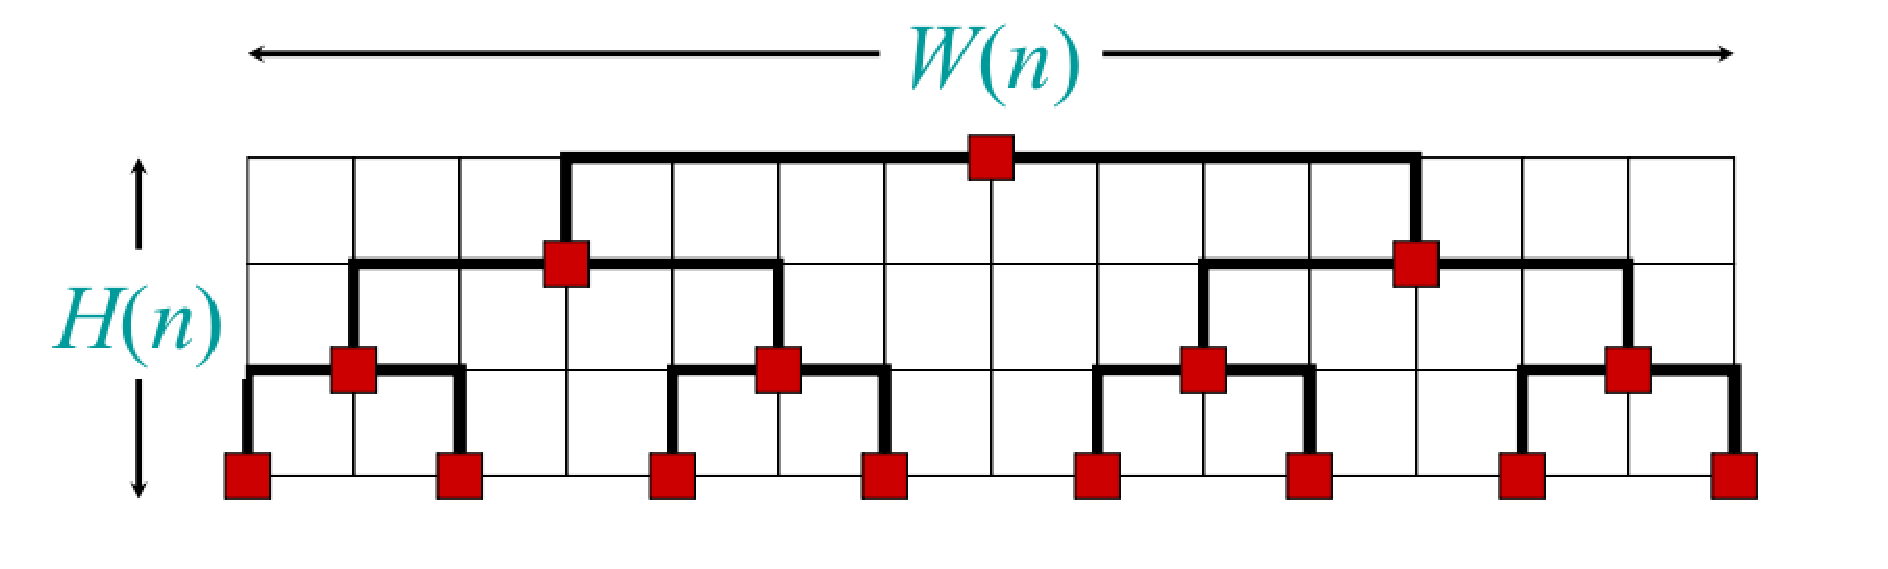
\includegraphics[width=4in]{lecture3/tree1.eps}
  \caption{Дерево}
  \label{fig:tree1}
\end{figure}

\begin{equation*}
  H(n) = H(n/2) + \Theta(1) = \Theta(\lg n)
\end{equation*}

\begin{equation*}
  W(n) = 2W(n/2) + \Theta(1) = \Theta(n)
\end{equation*}

\begin{equation*}
  \text{Площадь }= \Theta(n \lg n)
\end{equation*}

\begin{figure}[ht]
  \centering
  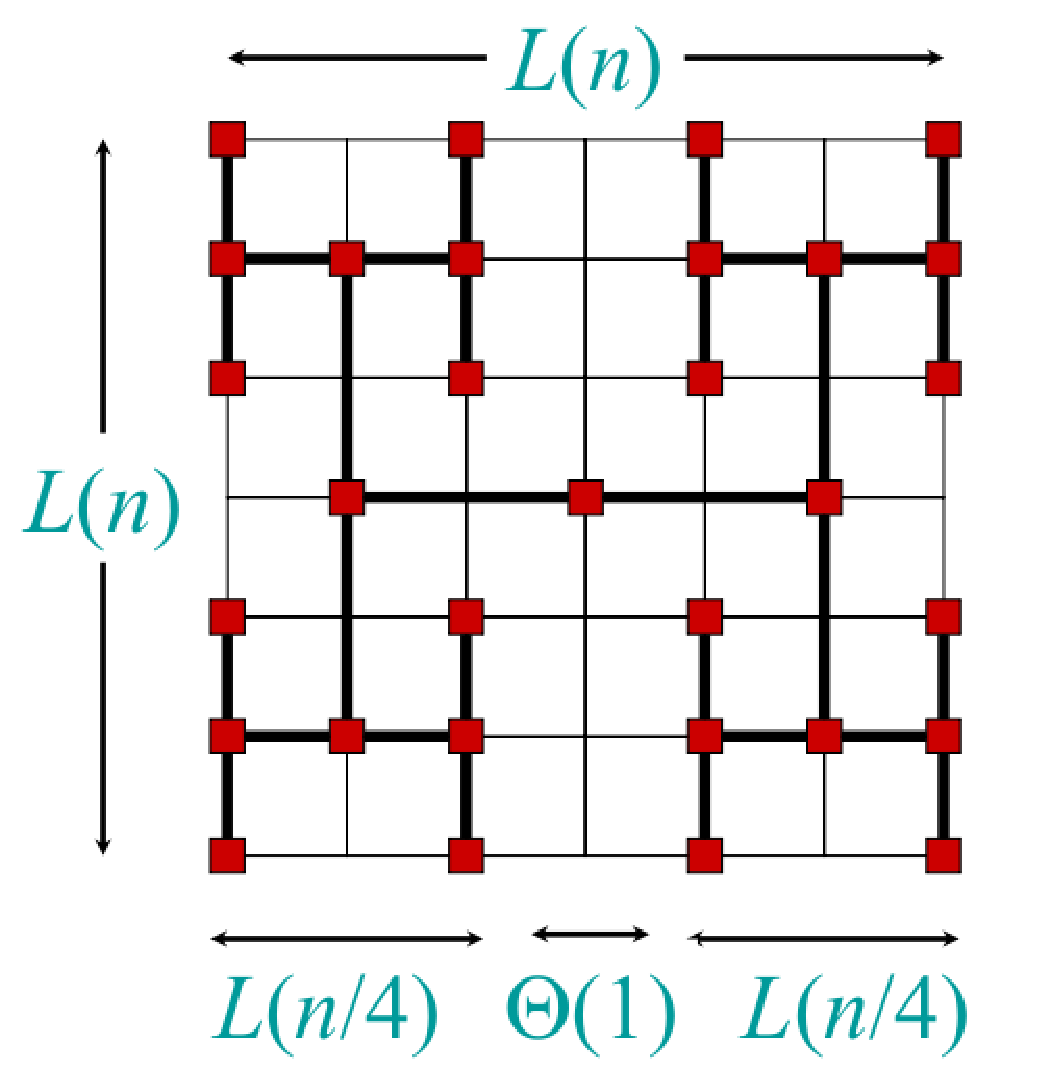
\includegraphics[width=3in]{lecture3/tree2.eps}
  \caption{Дерево 2}
  \label{fig:tree2}
\end{figure}

\begin{equation*}
  L(n) = 2L(n/4) + \Theta(1) = \Theta(\sqrt n)
\end{equation*}

\begin{equation*}
  \text{Площадь }= \Theta(n)
\end{equation*}

\section{Заключение}
\begin{itemize}
\item ``Разделяй и властвуй'' -- одна из нескольких мощных техник для разработки
  алгоритмов
\item Оценка времени выполнения этих алгоритмов сводится к рекуррентностям,
  которые легко решаются Основной теоремой
\item Стратегия ``Разделяй и властвуй'' часто позволяет получить весьма
  эффективные алгоритмы
\end{itemize}
\end{document}
